\textbf{Hvordan kommer data inn?}

Databasen vi har valgt tar utgangspunktet i et datasett som bruker data fra en undersøkelse på studenter fra to skoler i Portugal. For at ny data skal bli lagt inn i databasen, må det gjøres enda en undersøkelse ved enten de samme skolene eller en ny skole. Dataen må deretter legges inn via nettskjemaet med følgende felt på nettsiden:

\begin{itemize}
  \item Skole
  \item Kjønn
  \item Alder
  \item Mors-utdanning
  \item Fars-utdanning
  \item Reisetid
  \item Studietid
  \item Stryk
  \item Skolestøtte
  \item Ekstratimer (Betalt)
  \item Aktiviteter utenom faget
  \item Internett
  \item Romantisk forhold
  \item Familie Relasjon
  \item Fritid
  \item Gå ut med venner
  \item Alkohol i ukedagene
  \item Alkohol i helgen
  \item Helse
  \item Fravær
  \item Karakter semester 1
  \item Karakter semester 2
  \item Sluttkarakter
\end{itemize}

Totalt er det 22 felt som må fylles ut, mange av feltene vil ha standardverdier. I tillegg til nettskjemaet vil det være mulig å laste opp datasett i form av CSV eller JSON som har de samme kolonnene. Rader som er duplikater, vil ikke bli tatt hensyn til siden det er mulig å produsere de samme verdiene. Dette vil si at noen må manuelt legge til data via nettsiden for at dataen skal dukke opp i databasen, den vil ikke lytte etter endringer i datasettet via API-er.

Dersom ny data legges inn, som ikke samsvarer med strukturen som eksisterer, vil det ikke være noe problem. Skjemaløse databasemodeller er åpne for mindre rigide prosesser for innlegging av ny data, som er ønskelig ved potensielt varierende kilder.


\textbf{RIAK eller ETCD}

I prosjektet vårt har vi bestemt oss for å bruke ETCD, siden ETCD prioriterer konsistensen til dataen over tilgjengelighet. For dette prosjektet er det mye viktigere at dataen stemmer, enn å ha rask respons-tid. Hele hensikten med denne seksjonen er å forstå effekten studenters bakgrunn har på resultatene ved de forskjellige skolene, derfor må dataen være oppdatert. Siden CAP-teoremet gjelder i praksis kun når det oppstår en nodefeil, betyr det ikke at vi ofrer tilgjengelighet fullstendig, men det er mindre viktig i dette tilfellet enn konsistens. Til slutt er det merkverdig å nevne at Riak er mye mer omfattende enn ETCD, derfor blir det også foretrukket i prosjektet.


\textbf{Design av nøkkel}

På grunn av måten vi velger å oppdatere eksisterende data i databasen, blir nøklene designet på en måte som skiller mellom komponenter og ny studentdata. Komponentene er JSON-objektene som brukes til å vise data på nettsiden, mens studentdataen er rådata som er nyttig for å holde dataen oppdatert. Hvis en student legges til eller oppdateres, oppdateres også komponentene i databasen. Den generelle strukturen på nøkkelen vil derfor være et prefiks for inndeling, etterfulgt av kolon, etterfulgt av navn eller id.

Verdier relatert til komponenter vil ha en nøkkel med prefiks "component" etterfulgt av navnet på komponenten. Eksempel på en nøkkel for en komponent i vår KV-store:

  \textit{component:studentByFreeTime}

Verdier relatert til studenter vil ha nøkler med prefiks "student" etterfulgt av en 8-sifret id av typen Integer. Eksempel:
\textit{student:02381225}

KV-store vil dermed følge en lignende struktur:

\FigureCounter
\begin{figure}[H]
  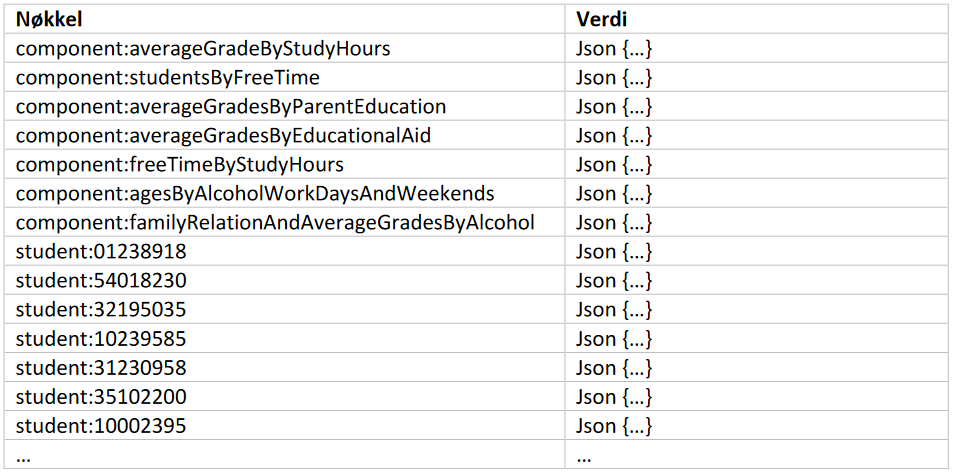
\includegraphics[width=\textwidth]{images/milepael2/tabellKVStore.png}
\end{figure}

\subsubsection{Design av dataobjekter og aggregeringer}

Vi har delt opp dataobjektene i to grupper: komponenter og student-data. Grunnen til denne oppdelingen er for å optimalisere ytelse ved uthenting og oppdatering av data. Oppdelingen gjør det mulig å oppdatere individuelle komponenter ved å kun lese fra student-dataen som endret seg. Da unngår man å hente alle student-dataene for å oppdatere alle komponentene, og som resultat gjør nettsiden færre kall til databasen.




